\section{System Architecture Overview}
\label{sec:sys_overview}

The system is to meant to be able to perform classification on the MNIST dataset, by using a TM model with 2000 clauses across 10 classes. The images in MNIST are $28 \times 28$ pixels large, meaning the feature vector $X$ is 784 bits long, and the literal vector (and action bit plane of each clause) will be 1568 bits long. This results in total model size of almost 4 MB. This not only far exceeds the NEORV32's default DMEM size of 8 kB, this also exceeds the total amount of available Block RAM (BRAM) available on the Artix-7 100T which is 607.5 kB. Memory is there a central design challenge in this work, which resulted in a multi-tier storage architecture, as shown in Figure \ref{fig:sys_arch}.

\begin{figure}[H]
    \centering
    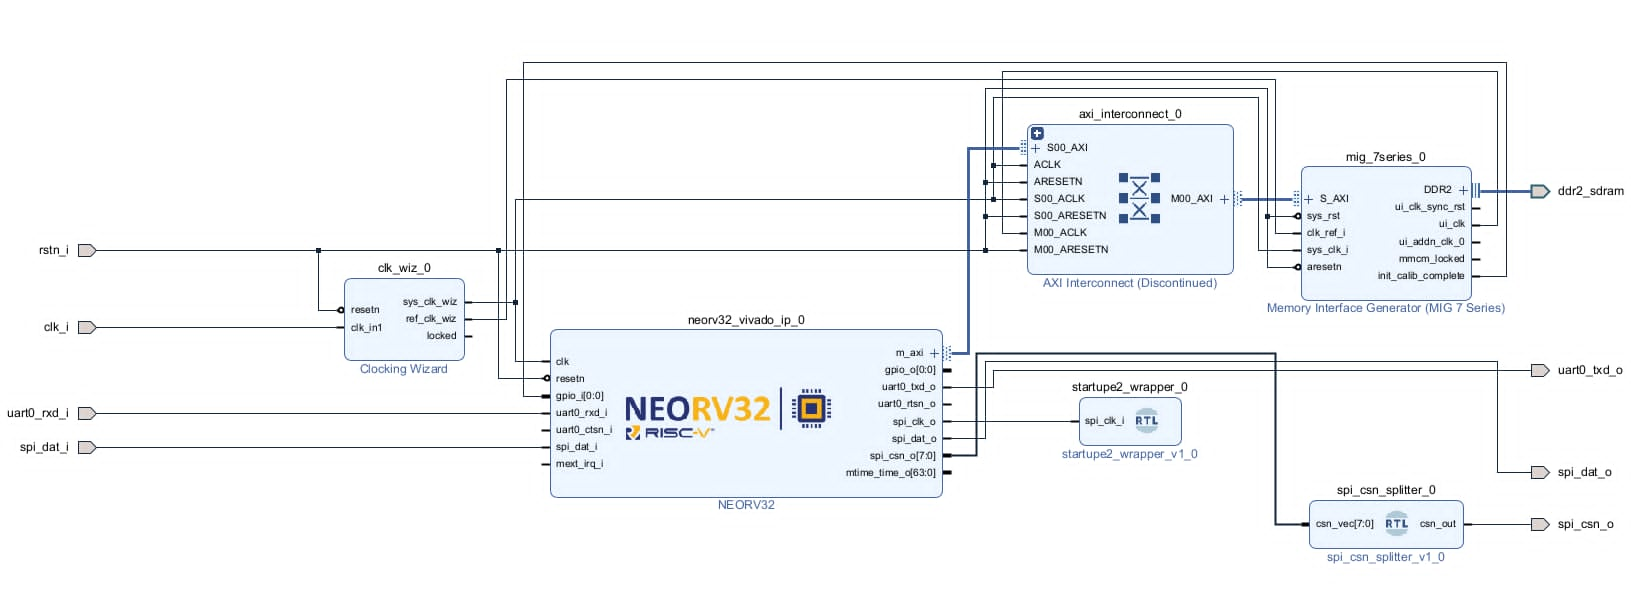
\includegraphics[width =1.2\textwidth]{Figures/blokk_diag.jpg}
    \caption{Block diagram of the full system, showing the NEORV32 processor 
    connected to DDR2 SDRAM via the AXI interconnect and MIG controller, and 
    to QSPI Flash via the SPI peripheral and STARTUPE2 wrapper. \textcolor{red}{MIDLERTIDIG, LAG I DRAW.IO}}
    \label{fig:sys_arch}
\end{figure}

The overall architecture is organized around three tiers of memory with distinct access characteristics. The trained model is stored persistently in on-board QSPI Flash, which survives power cycles but is too slow for direct inference use. At boot, the model is transferred from Flash into DDR2 SDRAM, which provides sufficient capacity for the full model and faster sequential access. During inference, model data is moved from DDR2 into the processor's internal DMEM, where clause evaluation is performed from fast on-chip storage.

The NEORV32 processor is connected to DDR2 through the XBUS interface, using a Wishbone-to-AXI4 bridge and a Xilinx MIG controller. QSPI Flash is accessed through the NEORV32 SPI peripheral. A Custom Functions Unit (CFU) is integrated directly into the CPU pipeline to accelerate clause evaluation using custom RISC-V instructions. Communication with a host PC is handled over UART at 921600 baud. The host sends booleanized input samples and receives predicted class labels together with cycle-accurate timing measurements.